
\documentclass[main.tex]{subfiles}
\begin{document}

\subsection{Objektově orientované programování}
\label{oop}
Objektově orientované programování (OOP) je programovací paradigma (styl, technika), založené na konceptu objektů, jež uchovávají data a kód, který by se měl vztahovat k datům objektu. Kód, jež je ve standardním smyslu funkcí, se v kontextu objektu nazývá metoda. Určitým protipólem k OOP je programování imperativní ( procedurální ). Základními pojmy OOP jsou:
\begin{itemize}
    \item Třída - šablona, podle které se následně vytváří objekt. Všechny objekty dané třídy ponesou stejné proměnné (stejný datový typ, pokud je rozlišován, a názvy proměnných), ale mohou v nich mít uložené jiné hodnoty. 
	\item Objekt - proměnná, která obsahuje další proměnné, tak jak byly nadeklarovány ve třídě. Prakticky pomáhá k abstrakci jednoduchých datových typů do větších, člověku přístupnějších, datových celků.
		\begin{figure}[h]
			\centering
			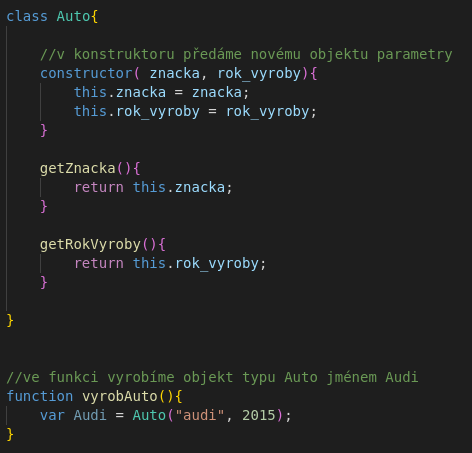
\includegraphics[width=.6\textwidth]{./images/oop/class_audi.png}
			\caption{Rozdíly mezi objektem a třídou}
		\end{figure}
		Nejprve je vytvořena třída Auto, která obsahuje proměnné znacka, rok\_vyroby, model. Poté je vytvořen samotný objekt \textit{Audi}, který v sobě uchovává všechny proměnné, k nimž lze přistupovat. (implementace v javascriptu)
    \item Zapouzdření - k datům objektu je typicky zakázáno přistupovat jinak, než přes jeho rozhranní - funkce ( v kontextu objektů nazývané metody). Tyto metody se obvykle nazývají get a set.
	\item Dědičnost - pro možnost větší abstrakce slouží dědičnost. Objekt může být potomkem jiného objektu. Tehdy přebírá jeho vlastnosti - data a metody. Tyto vlastnoti jsou dále součástí objektu a lze k nim přistupovat běžným způsobem.
		%\img{} %obrazek s dedenim tridy
	\item Polymorfismus - umožňuje různým objektům, které mají společného předka, aby byla zavolána metoda přes tohoto předka. Implementace dané funkce se v potomcích typicky liší.
		%\img{}
		Dalším druhem polymorfismu (parametrický) je volání funkce pro různé datové typy. Příklad z jazyka c++, ve kterém to umožňuje použití šablon.
		\begin{figure}[h]
			\centering
			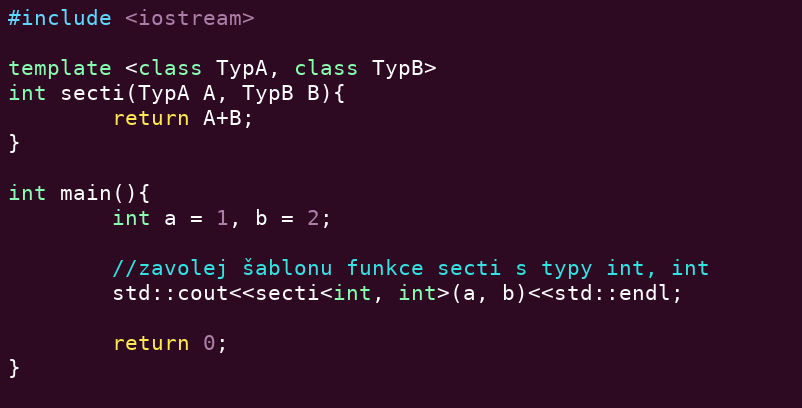
\includegraphics[width=.8\textwidth]{./images/oop/prototype.png}
			\caption{Příkald parametrického polymorfismu.}
		\end{figure}
	%	Zahrneme-li toto pravidlo do HTML, všechny nadpisy 3. úrovně budou modrou barvou, velikosti 10 pixelů a podtržené.
		%\img{}
	\cite{web:wik:en:oop}
\end{itemize}
\end{document}
